%!TEX root = Tesi.tex

\section{Ambiente di sviluppo}
\subsection{Introduzione}
\'E stato scelto di sviluppare l'intero progetto di tesi in ambiente UNIX, usando come sistema operativo Linux, nello specifico la distribuzione di Ubuntu 17.04 a 64 bit denominata Zesty Zapus. Questa decisione è stata presa per integrare al meglio i progetti ed il codice già esistente e per creare una base di sviluppo futura che sia Open Source\footnote{Qualità di un sistema che consiste nell'essere di libero uso e riutilizzabile senza alcun costo, per ampliarne funzionalità e caratteristiche} e liberamente utilizzabile senza alcun vincolo di licenza. Non è stata comunque una decisione immediata perché il RedBear Nano2 integra un Soc\footnote{Sistem on a Chip, è un particolare circuito integrato che in un solo chip contiene un sistema completo} progettato dalla società Nordic Semiconductor, chiamato \lq\lq nRF52832\rq\rq, la quale mette a disposizione vari Tool, funzionalità e IDE di sviluppo per questo chip ideati e creati  per funzionare unicamente in ambiente Windows; fortunatamente esistono vari progetti e guide abbastanza dettagliate reperibili online, alcune delle quali supportate direttamente dalla Nordic stessa, che aiutano a settare ed integrare il materiale già esistente anche in ambiente UNIX.
Rimangono comunque delle forti limitazioni nello sviluppo degli applicativi per Nano2 su Linux, primo fra tutti la mancanza della possibilità di un ambiente di Debug che permetta l'analisi istruzione per istruzione del codice in esecuzione sul dispositivo, con la relativa possibilità di visualizzazione dei valori delle varie variabili durante l'esecuzione; questa limitazione è stata in parte sopperita utilizzando l'interfaccia UART, utilizzandola per inviare stringhe contenenti informazioni su quali parti del codice fossero o meno state realmente eseguite ed il valore di alcune variabili di interesse nelle varie fasi dell'esecuzione dell'applicativo sviluppato. 
Questa incompatibilità ha rallentato il processo di sviluppo su Linux ma non lo ha reso impossibile, ne tanto meno ne ha limitato le potenzialità.

\subsection{Installazione GNU toolchain}\label{inst_gnu_toolchain}
Prima di iniziare a scrivere codice, è necessario installare dei componenti software che permettano di compilare in linguaggio macchina ARM il codice da noi prodotto.
Quello che ci serve è un compilatore chiamato \emph{GNU toolchain for ARM Cortex-M} scaricabile gratuitamente dal sito ufficiale di \lq arm.developer\rq. \cite{armweb} Una volta scaricato ed estratto il pacchetto, bisognerà aggiungere al PATH di sistema la seguente directory:

\begin{minted}{bash}
<directory estratta>/gcc-arm-none-eabi-6-2017-q2-update/bin
\end{minted}

Per compiere questa operazione in Ubuntu, basterà aprire una finestra del terminare BASH ed eseguire il comando:

\begin{minted}[breaklines]{bash}
echo 'export PATH=\$PATH:<directory estratta>/gcc-arm-none-eabi-6-2017-q2-update/bin' >> ~/.profile 
\end{minted}

ovvero aggiungere al file .profile il percorso al compilatore, il quale sarà aggiunto poi in automatico alla variabile di sistema PATH; questo permetterà di invocare i comandi di compilazione da qualunque punto del sistema, senza dover richiamare il percorso al compilatore.
\'E possibile verificare se il procedimento è stato eseguito con successo eseguendo il seguente comando al terminale:

\begin{minted}{bash}
arm-none-eabi-gcc --version
\end{minted}
che deve restituire la versione del compilatore installata.

Un altro componente essenziale da aver installato è il compilatore \emph{GNU make}, che normalmente è già presente sulla maggior parte delle distribuzioni UNIX. Se così non fosse, per quanto riguarda Ubuntu, si installa semplicemente eseguendo il comando:

\begin{minted}{bash}
sudo apt-get install build-essential checkinstall
\end{minted}

\subsection{Configurazione SDK}
L'SDK\footnote{Software Development Kit}, ovvero l'insieme di tutte le funzioni di libreria necessarie per creare applicazioni da eseguire sul Nano2, è liberamente scaricabile dal sito della Nordic Semiconductor \cite{sdkweb} ; La versione utilizzata per questo progetto è la 14.1.0 che è creata per essere utilizzata sul Chip nRF52832.
La struttura di questa SDK è molto rigida, tutti i progetti contenuti al suo interno fanno riferimento ai vari file contenuti nell'SDK con un percorso assoluto; è meglio quindi non modificarne la struttura per non avere problemi di compilazione in futuro.
Scaricata ed estratta in una directory a piacimento, va impostato il percorso alla toolchain ARM, installata nel capitolo \ref{inst_gnu_toolchain}, andandolo a impostare nel file makefile.posix che si trova nella cartella: 

\begin{minted}{text}
<SDK>/components/toolchain/gcc
\end{minted}
dove \textless SDK\textgreater  è la root dell'SDK estratto.

Aprendo il file con un semplice editor di testo, cambiare i 3 campi riportati come segue:

\begin{minted}{text}
GNU_INSTALL_ROOT := <directory estratta>/gcc-arm-none-eabi-6-2017-q2-update/bin/
GNU_VERSION := 6.3.1
GNU_PREFIX := arm-none-eabi
\end{minted}

Nella SDK si trovano anche molti progetti di esempio, da cui è essenziale partire per sviluppare un nuovo programma; ogni progetto di esempio contiene svariati file sorgente da compilare e linkare. Per rendere semplice la compilazione è fornito un Makefile, ovvero un file che contiene tutte le istruzioni per la compilazione del progetto e che integra regole di dipendenza e regole di interpretazione, utilizzate per conoscere quali sono i file utilizzati nel progetto, con il relativo percorso, garantendo una compilazione esente da errori e solo di quei file sorgente che sono stati modificati dall'ultima compilazione.

Da questo punto è possibile compilare un progetto di esempio direttamente da terminale, per verificare che i passi compiuti fin'ora siano stati eseguiti correttamente; portandosi nella cartella del progetto \lq blinky\rq e successivamente nella sotto cartella \emph{armgcc}; qui invocando il comando \emph{make} si avvierà la compilazione che se avrà successo creerà una sotto cartella chiamata \_build contenete il file nrf52832\_xxaa.hex, che è il nostro programma compilato in linguaggio macchina ARM che dovrà essere poi scritto sulla memoria del Nano2 per essere eseguito.
Per scrivere il file sulla memoria del Nano2 basterà copiarlo all'interno della periferica usb che viene rilevata dal pc quando lo si connette tramite la board DAPLink v1.5 .
\subsubsection{Configurazione piedinatura Nano2}
Il dispositivo della società RedBear chiamato Nano2 che viene utilizzato in questa tesi, non è uno dei dispositivi ufficialmente supportati dalla SDK; Bisogna quindi prendere una delle varie board che vengono ufficialmente supportate e cambiarne la piedinatura, ovvero l'associazione tra una specifica periferica, come il led, o una specifica funzionalità, ad esempio UART, e il relativo pin sul chip. 
\'E stato scelto di prendere la board di sviluppo PCA10040 ed il relativo file di configurazione pca10040 e adattarne la piedinatura con quella dichiarata dalla Redbear, mostrata in figura \ref{nano2_pins}

\begin{figure}[H]
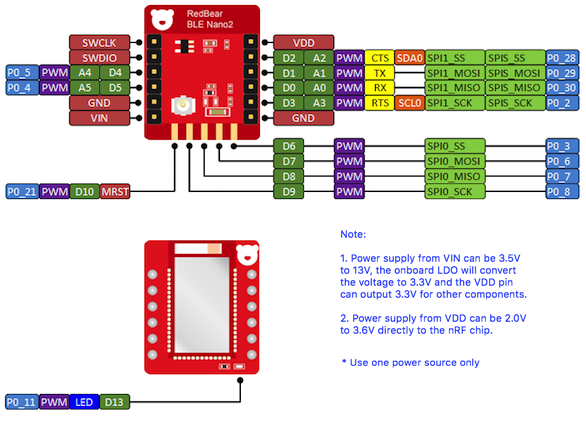
\includegraphics[width=350pt]{nano2_pins}
\centering
\caption{Piedinatura del modulo Nano2}
\label{nano2_pins}
\end{figure}
ad esempio, qui si ha a disposizione solo 1 led, connesso al pin 11, mentre sulla board PCA10040 se ne avevano 4. Bisognerà cambiare quindi il numero totale di led da 4 a 1 ed il pin dell'unico led con il valore 11.
Dopo aver modificato correttamente questo file, tutte le modifiche saranno automaticamente aggiornate per tutti gli esempi contenuti nell'SDK, andando a selezionare per ogni progetto il makefile contenuto nella cartella che riporta il nome della board PCA10040.
Per l'esempio del lampeggio del led, il percorso per raggiungere il makefile corretto sarà quindi:

\begin{minted}{text}
<SDK>/examples/peripheral/PCA10040/blank/armgcc/
\end{minted}

\subsubsection{Softdevice}
Progetti più complessi di un semplice lampeggio di un led, come tutti i progetti che permettono lavorare con il BLE, necessitano che assieme al codice del programma venga scritto sul dispositivo dell'altro codice preconfezionato; questo ulteriore codice, chiamato \emph{Softdevice} non è altro che un insieme di funzioni di libreria che vengono fornite già compilate e che sono utilizzabili dal nostro codice per svolgere le operazioni più complesse utilizzando poche righe di codice. Esistono varie versioni del softdevice, diverse per funzionalità e compatibilità con i chip; per tutti le applicazioni sviluppate è stata usata la versione S132.
Se si sta sviluppando un progetto che utilizza tali funzioni, prima di andare a scrivere il file .hex sul Nano2 bisognerà unirlo con il softdevice, che viene fornito nella SDK (<SDK>/components/softdevice/s132/hex), utilizzando una utility scaricabile dal sito della Nordic, chiamata \lq mergehex\rq, e disponibile per tutti i Sistemi Operativi.
Per velocizzare il processo di unione dei due file .hex e successiva scrittura sul Nano2 è stato creato uno script di bash che automatizza tutto il processo:

\begin{minted}{text}
#!/bin/bash

SOFTDEVICE=/home/utente/SoftDevices/s132_nrf52_5.0.0/s132_nrf52_5.0.0_softdevice.hex
SORGENTE=nrf52832_xxaa.hex 
OUTPUT=toflash.hex
USB_PROG=/media/utente/DAPLINK

mergehex -m ${SORGENTE} ${SOFTDEVICE} -o ${OUTPUT}

echo "Flashing to ${USB_PROG} ..."
cp ./${OUTPUT} ${USB_PROG}/{OUTPUT}
\end{minted}

\subsection{Installazione IDE}
Anche se non strettamente necessario ai fini dello sviluppo, un ambiente grafico per la scrittura del codice (IDE) è consigliato, dato il gran numero di righe di codice che può contenere un applicativo. Eclipse, l'IDE di sviluppo utilizzato in questa tesi, è un ambiente di sviluppo integrato multi-linguaggio e multipiattaforma sviluppato in Java dalla \emph{Eclipse Foundation}, distribuito liberamente e gratuitamente.
Oltre all'ide di base, nella versione per sviluppatori C,C++ vanno aggiunti vari pacchetti per permettere lo sviluppo sui dispositivi integrati con processore ARM; per facilitare le operazioni di aggiunta e settaggio di questi pacchetti esistono delle versioni di Eclipse modificate che integrano tutti questi pacchetti; queste versioni modificate è scaricabile gratuitamente dal repository GitHub \emph{gnu-mcu-eclipse} \cite{gnueclipseweb}. Scaricato ed estratto in una directory a piacimento sarà già pronto per essere utilizzato per sviluppare applicazioni per il Nano2.
\subsubsection{Importare un esempio in Eclipse}
Per inziare a sviluppare o testare uno dei vari esempi presenti nell'SDK utilizzando Eclipse, bisogna prima importarlo nell'ambiente di lavoro. 
Per fare ciò bisogna creare un nuovo progetto in Eclipse che si basi su un Makefile esistente.

\begin{minted}{text}
File -> Makefile Project with Existing Code
\end{minted}
andando poi a impostare come percorso la cartella che contiene il makefile del progetto; come toolchain bisognerà settare \lq ARM Cross GCC\rq .

\begin{figure}[H]
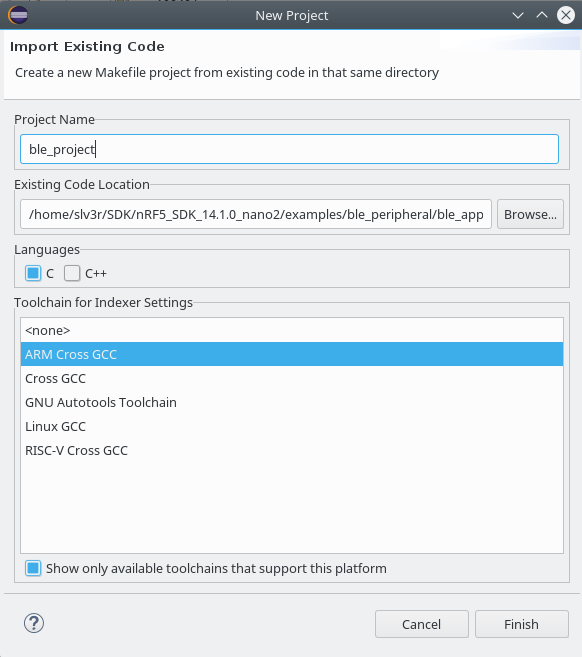
\includegraphics[width=300pt]{new_makefile_project}
\centering
\caption{Creazione di un nuovo progetto da Makefile}
\label{makefile_proj}
\end{figure}

Nella schermata dei progetti di eclipse apparirà il progetto appena creato, vedremo però solo il file Makefile; si deve importare manualmente il file main.c andando prima a creare una nuova cartella virtuale, tramite il percorso New -\textgreater  Folder e nella schermata selezionare Advanced e successivamente Virtual Folder. Poi tramite tasto destro sulla cartella -\textgreater  import andare a selezionare il file main.c che è situato nella cartella principale del progetto.

\begin{figure}[H]
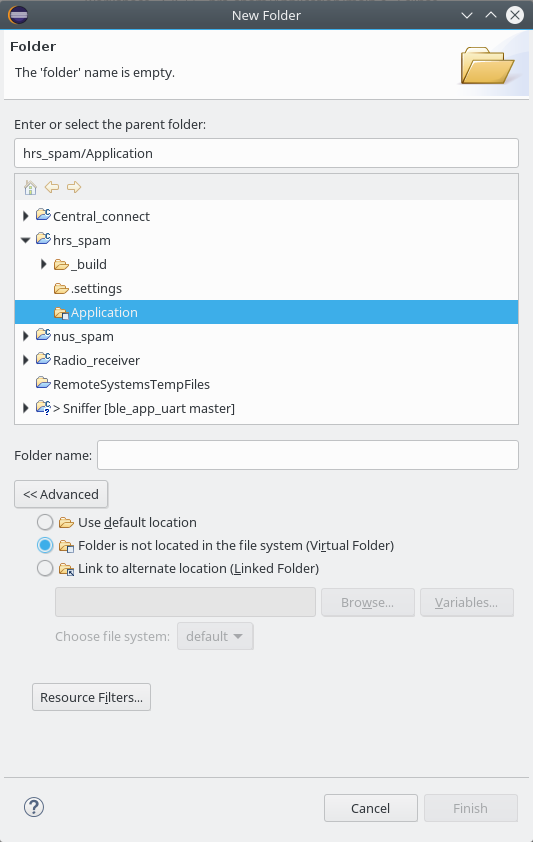
\includegraphics[width=270pt]{new_folder_eclipse}
\centering
\caption{Creazione di una cartella virtuale nel progetto, che conterrà il file main.c}
\label{makefile_proj}
\end{figure}

L'ultima operazione da compiere prima di poter compilare tramite Eclipse è settare il comando di compilazione; tramite tasto destro sulla cartella del progetto, visualizzata a lato sinistro, e selezionando Properties. Si aprirà una nuova schermata in cui si deve selezionare C/C++ Build ed impostare il campo Build Command come segue: 

\begin{minted}{text}
make VERBOSE=1
\end{minted}
Questo, oltre ad invocare il comando corretto di compilazione, crea un output di tipo \lq verbose\rq dal quale Eclipse ottiene le informazioni sui percorsi dei vari file da cui dipende il main, andando quindi ad eliminare tutti gli errori sintattici che erroneamente l'IDE evidenzia.

\begin{figure}[H]
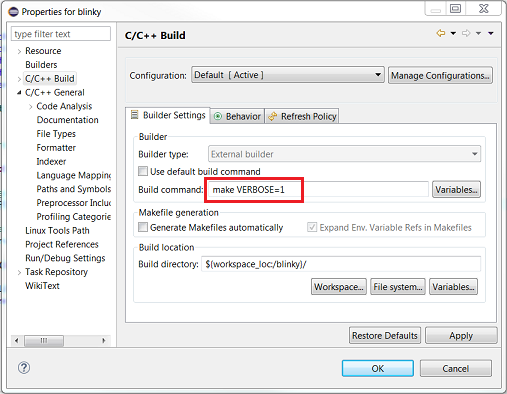
\includegraphics[width=350pt]{verbose_eclipse}
\centering
\caption{Impostazione del comando di compilazione su Eclipse}
\end{figure}

